\chapter{Supplementary materials for:\\An automated, objective and open source tool for stream threshold selection and upstream riparian corridor delineation}
\label{appendixA}

\section{Supplementary computer code and data}
\label{Supplementary computer code and data}

An R-script ``ATRIC: Automated Accumulation Threshold selection and RIparian Corridor delineation'' is available as a supplementary computer code with the digital version of this thesis that can also be downloaded from: \href{https://github.com/AvitBhowmik/ATRIC}{https://github.com/AvitBhowmik/ATRIC}. To allow for reproducibility, sample data was made available from the following online repositories:\\\href{http://doi.pangaea.de/10.1594/PANGAEA.825001}{http://doi.pangaea.de/10.1594/PANGAEA.825001},\\\href{https://github.com/AvitBhowmik/ATRIC}{https://github.com/AvitBhowmik/ATRIC}.

\newpage

\begin{landscape}
      
\section{Supplementary figures}
\label{Supplementary figures}

\begin{figure}[h!]
  \centering
  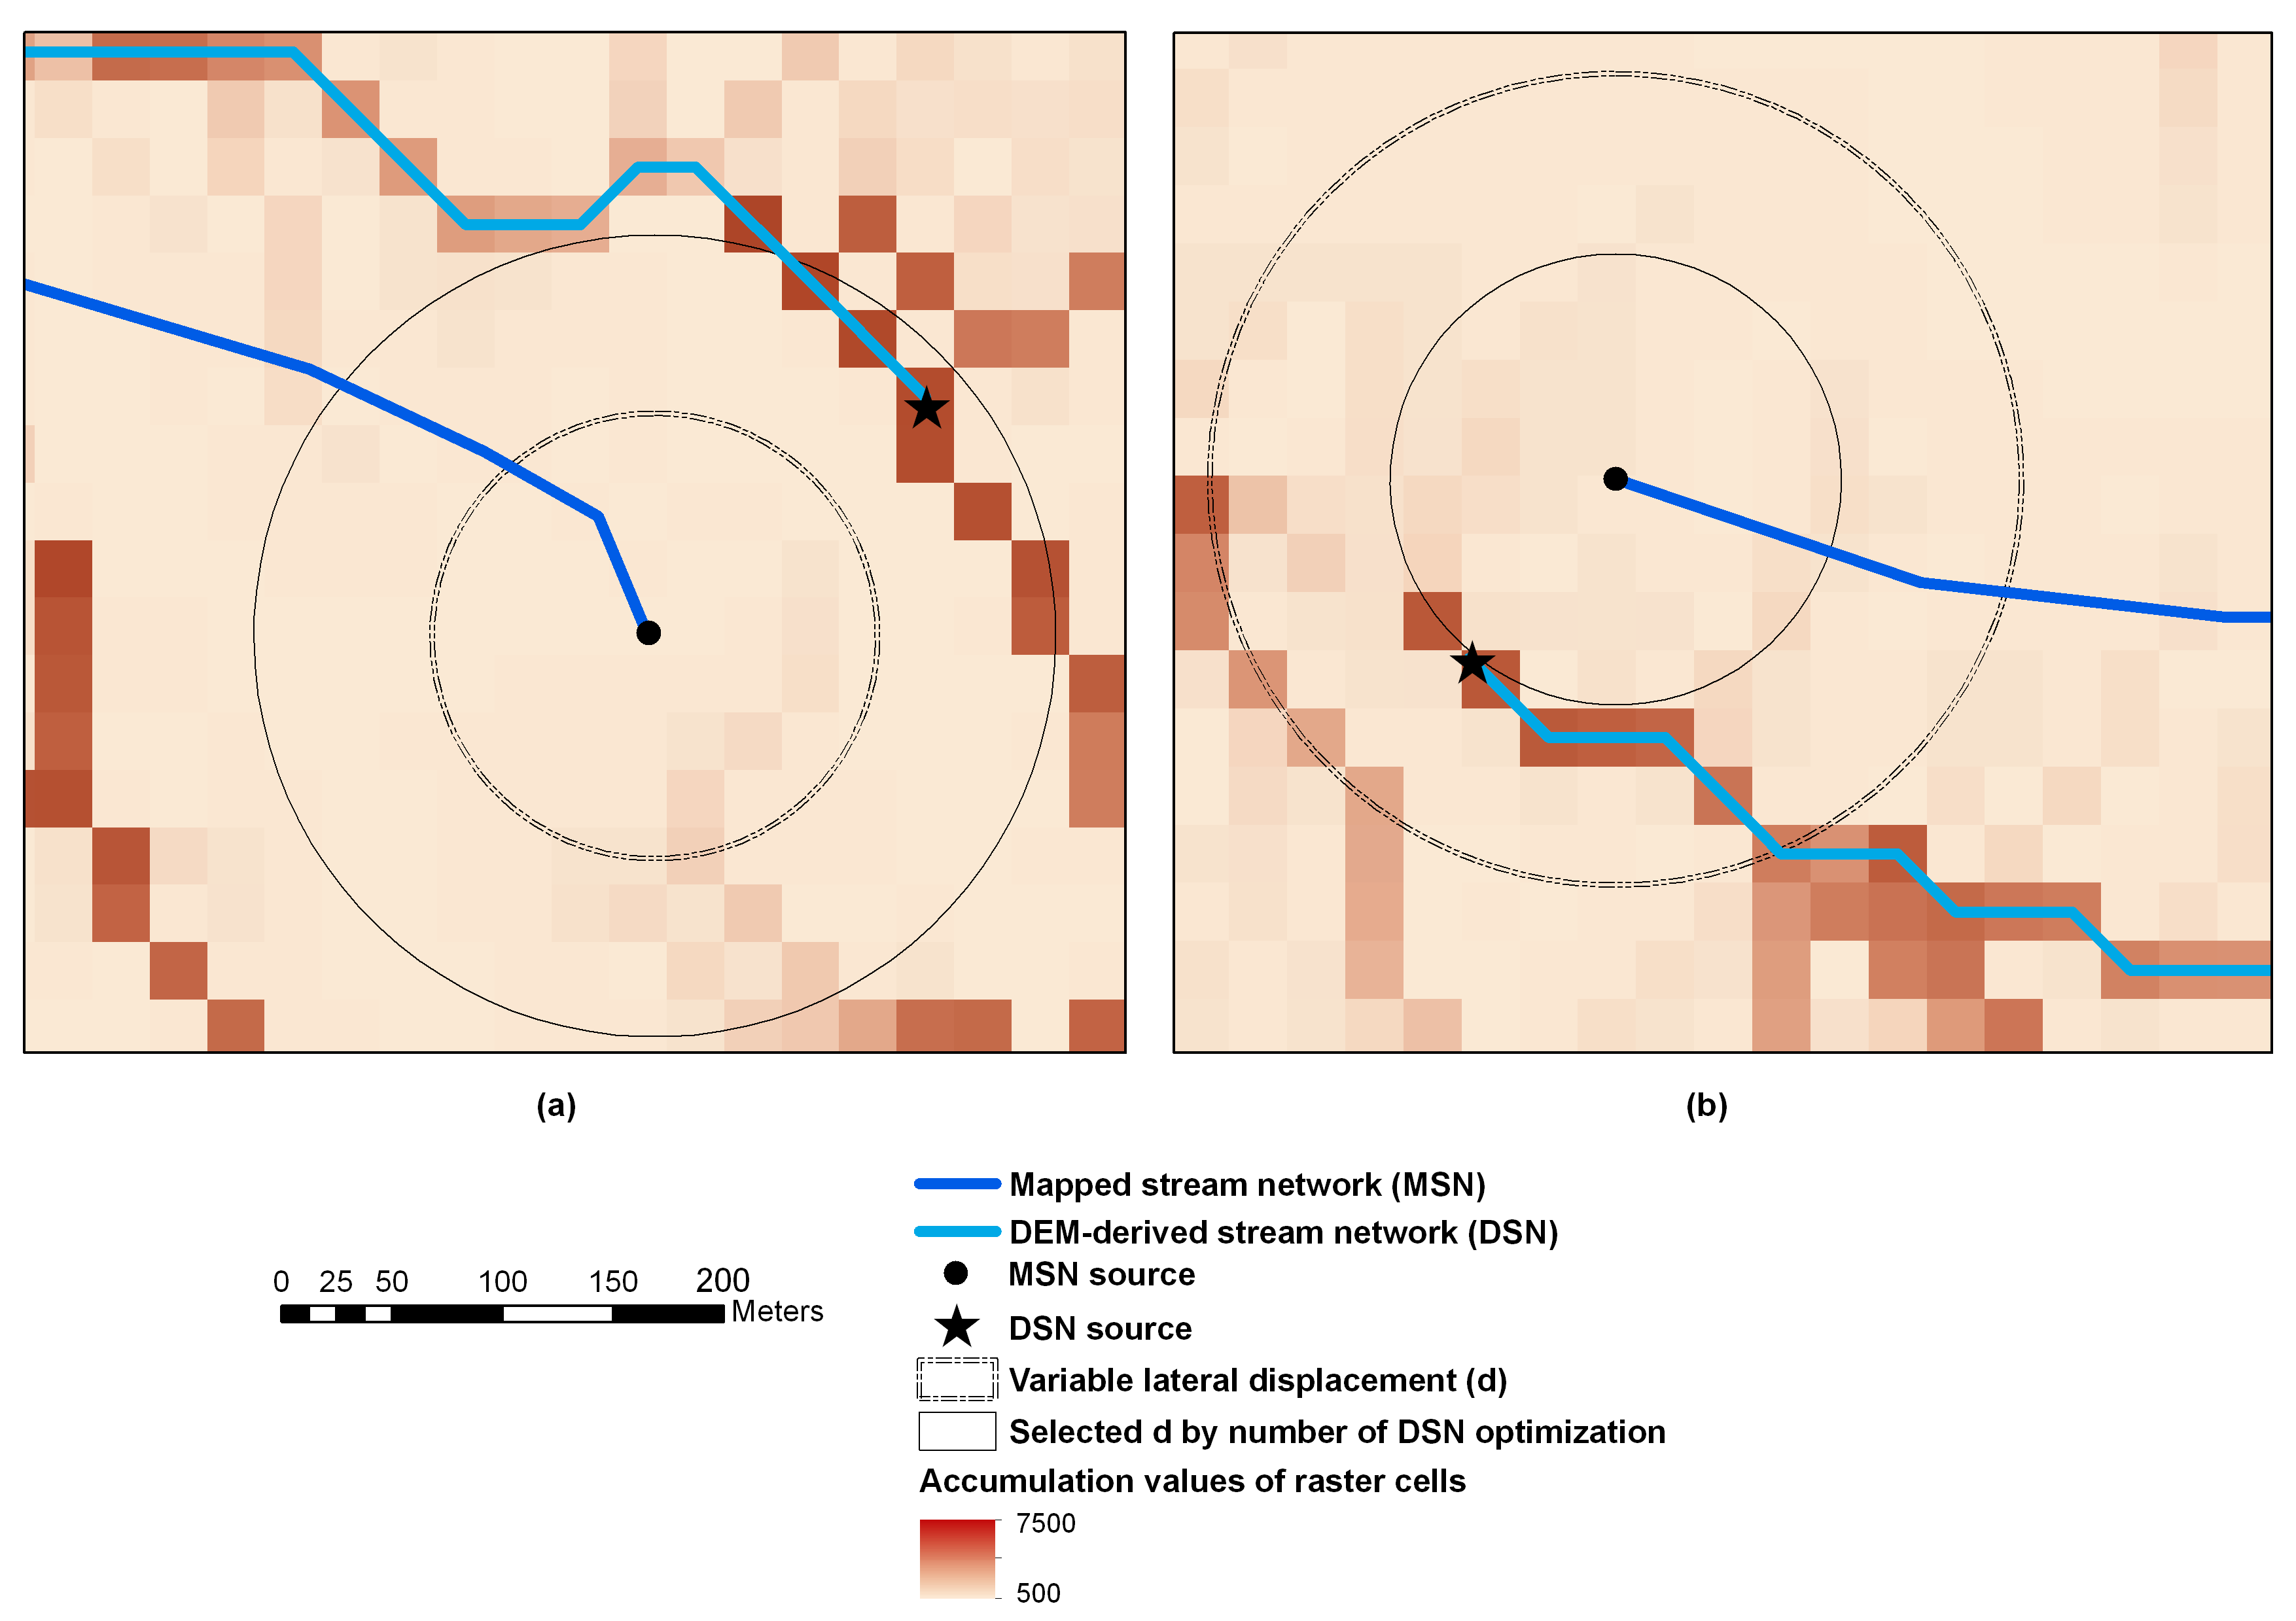
\includegraphics[width=0.71\linewidth]{Figures/Fig_S1_1.png}
  \caption{Variable lateral displacements ($d$) search buffers and selected d by optimizing number of digital elevation model (DEM)-derived stream cells ($n_{DS}$) optimization. When variable $d$s were (a) lower and (b) higher than the selected $d$ a lower and higher accumulation thresholds (AT), respectively, were obtained than the AT obtained by the selected $d$.}
  \label{Fig_A_1}
\end{figure}

\end{landscape}

\begin{figure}[h!]
  \centering
  \hspace{-1cm} 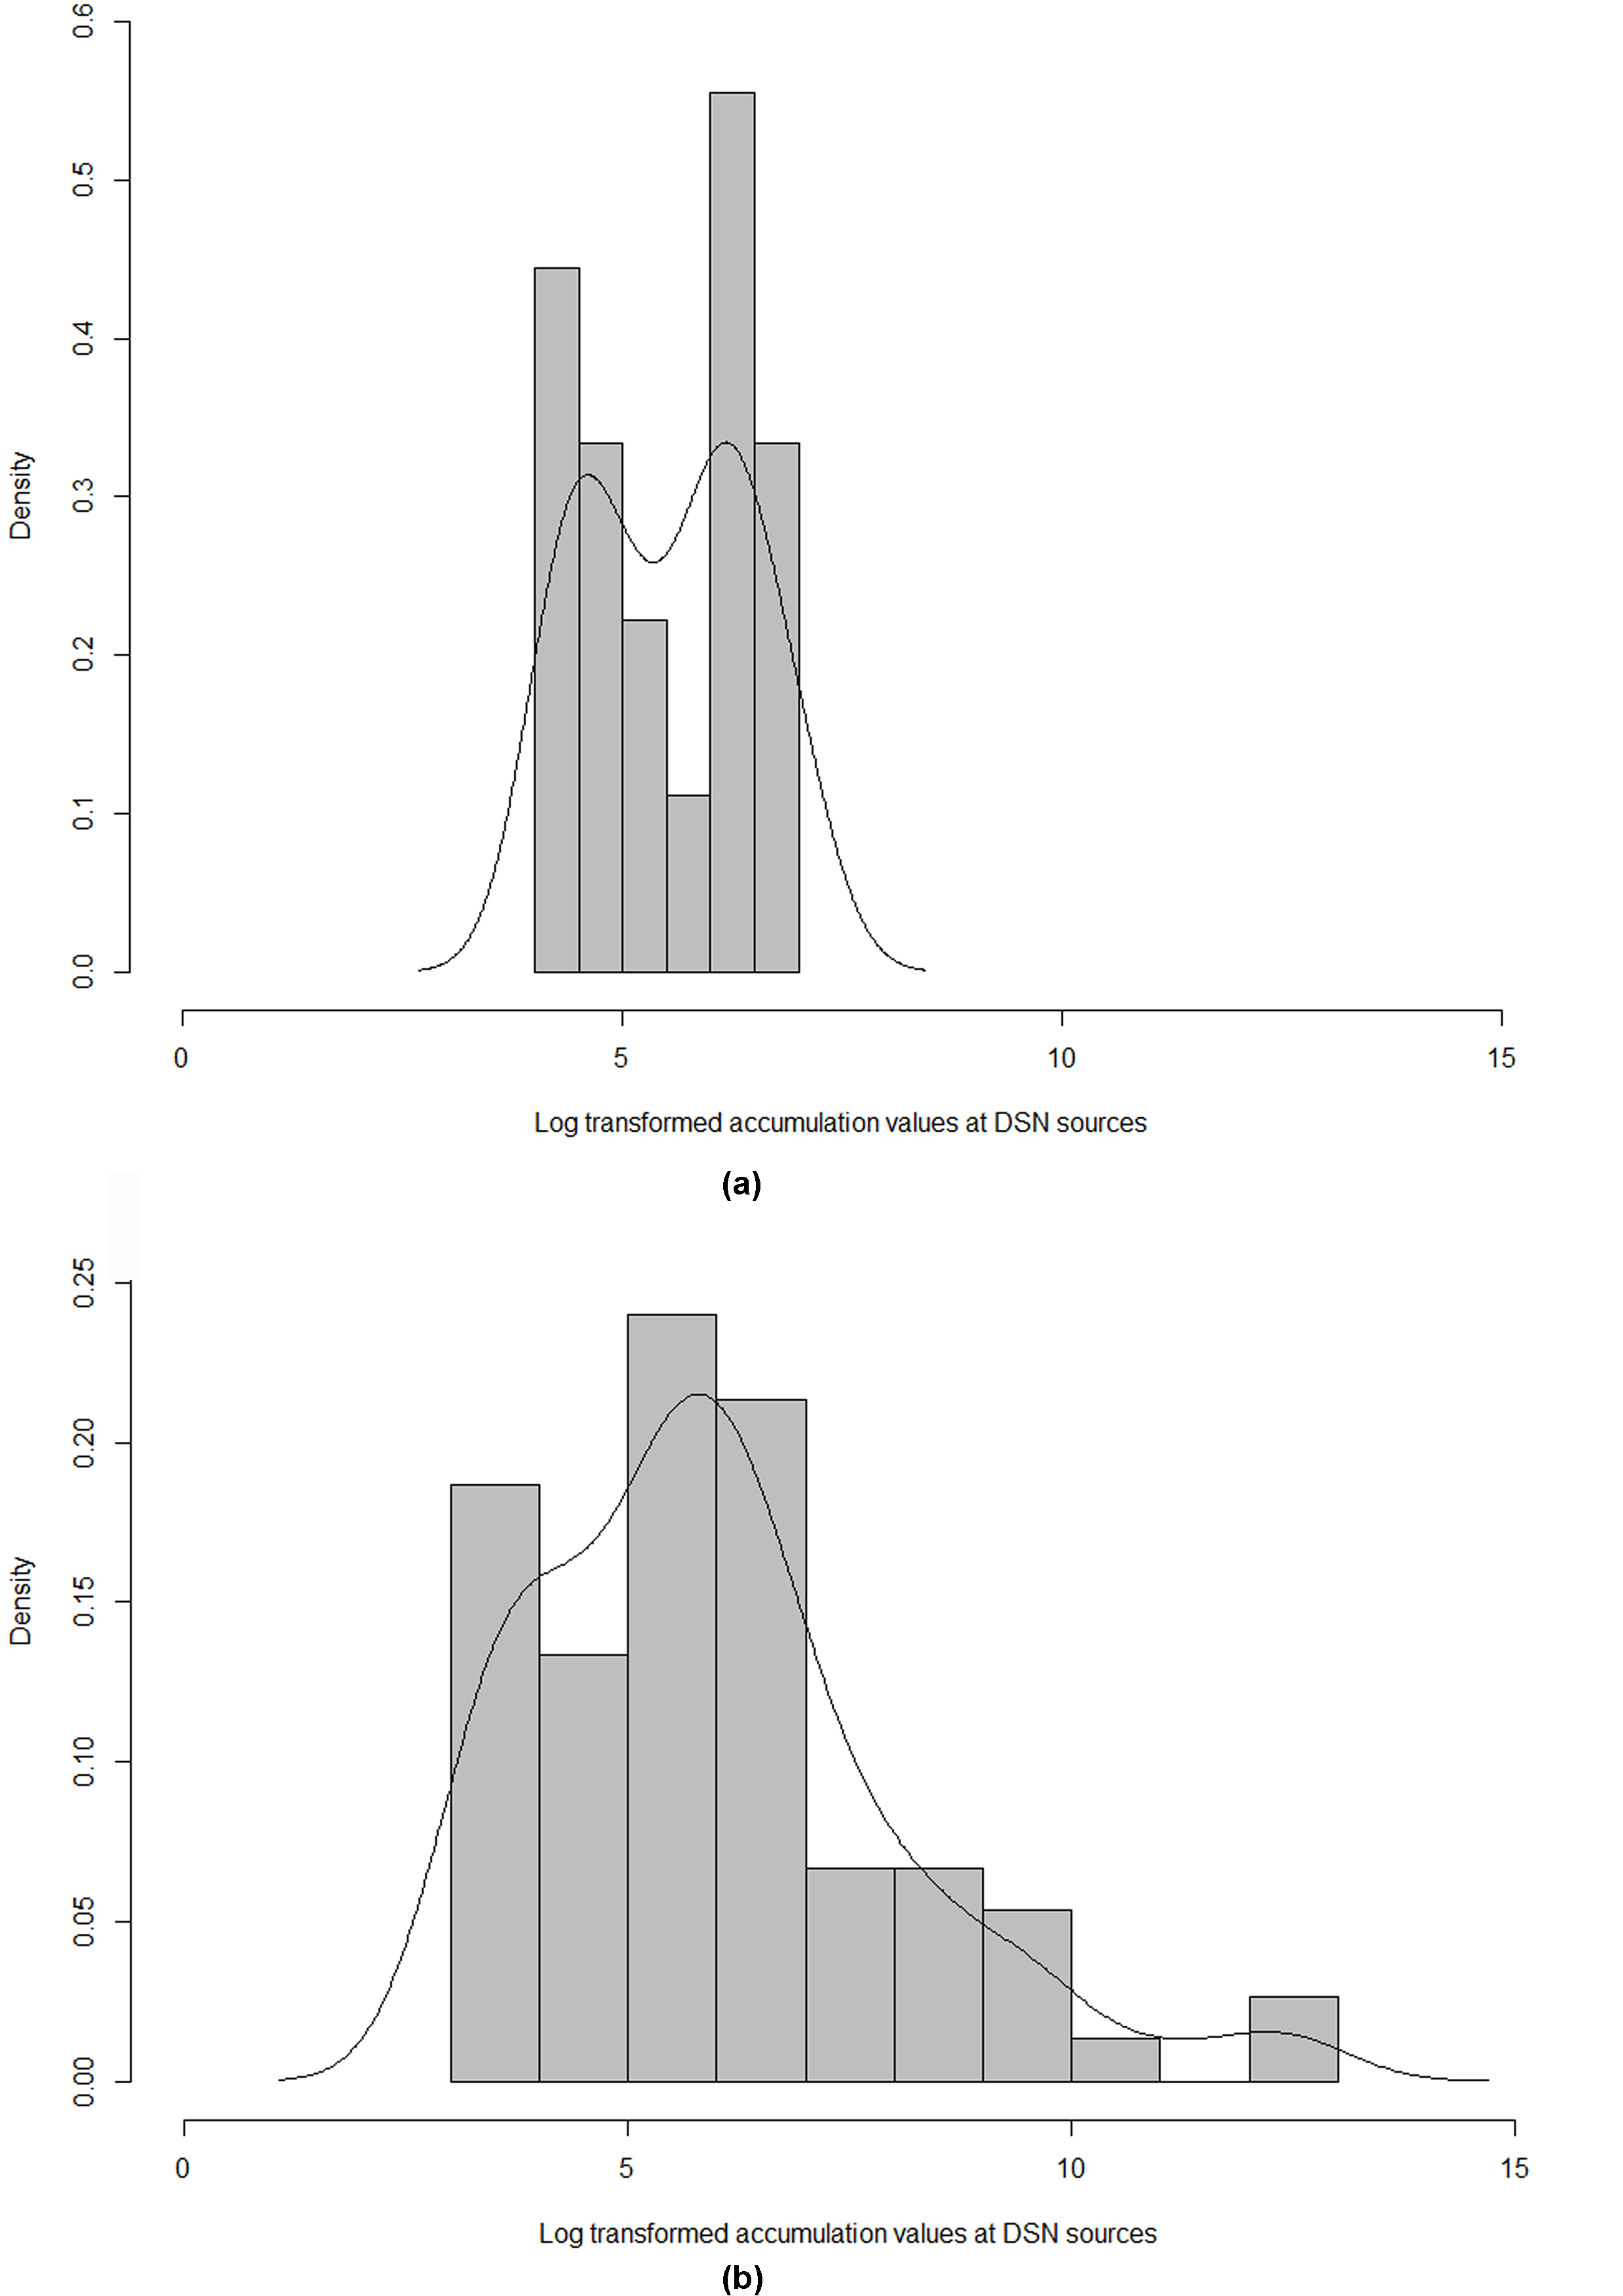
\includegraphics[width=1.1\textwidth]{Figures/Fig_S1_2.png}
  \caption{The histogram and Kernel density plots showing the distribution of the log transformed accumulation values at sources of the digital elevation model (DEM)-derived stream networks (DSN) obtained by the selected lateral displacement ($d$) search buffer in the (a) Hessen watershedand (b) state Thüringen.}
  \label{Fig_A_2}
\end{figure}

\begin{landscape}

\begin{figure}[h!]
  \centering
  \vspace{-1.3cm} 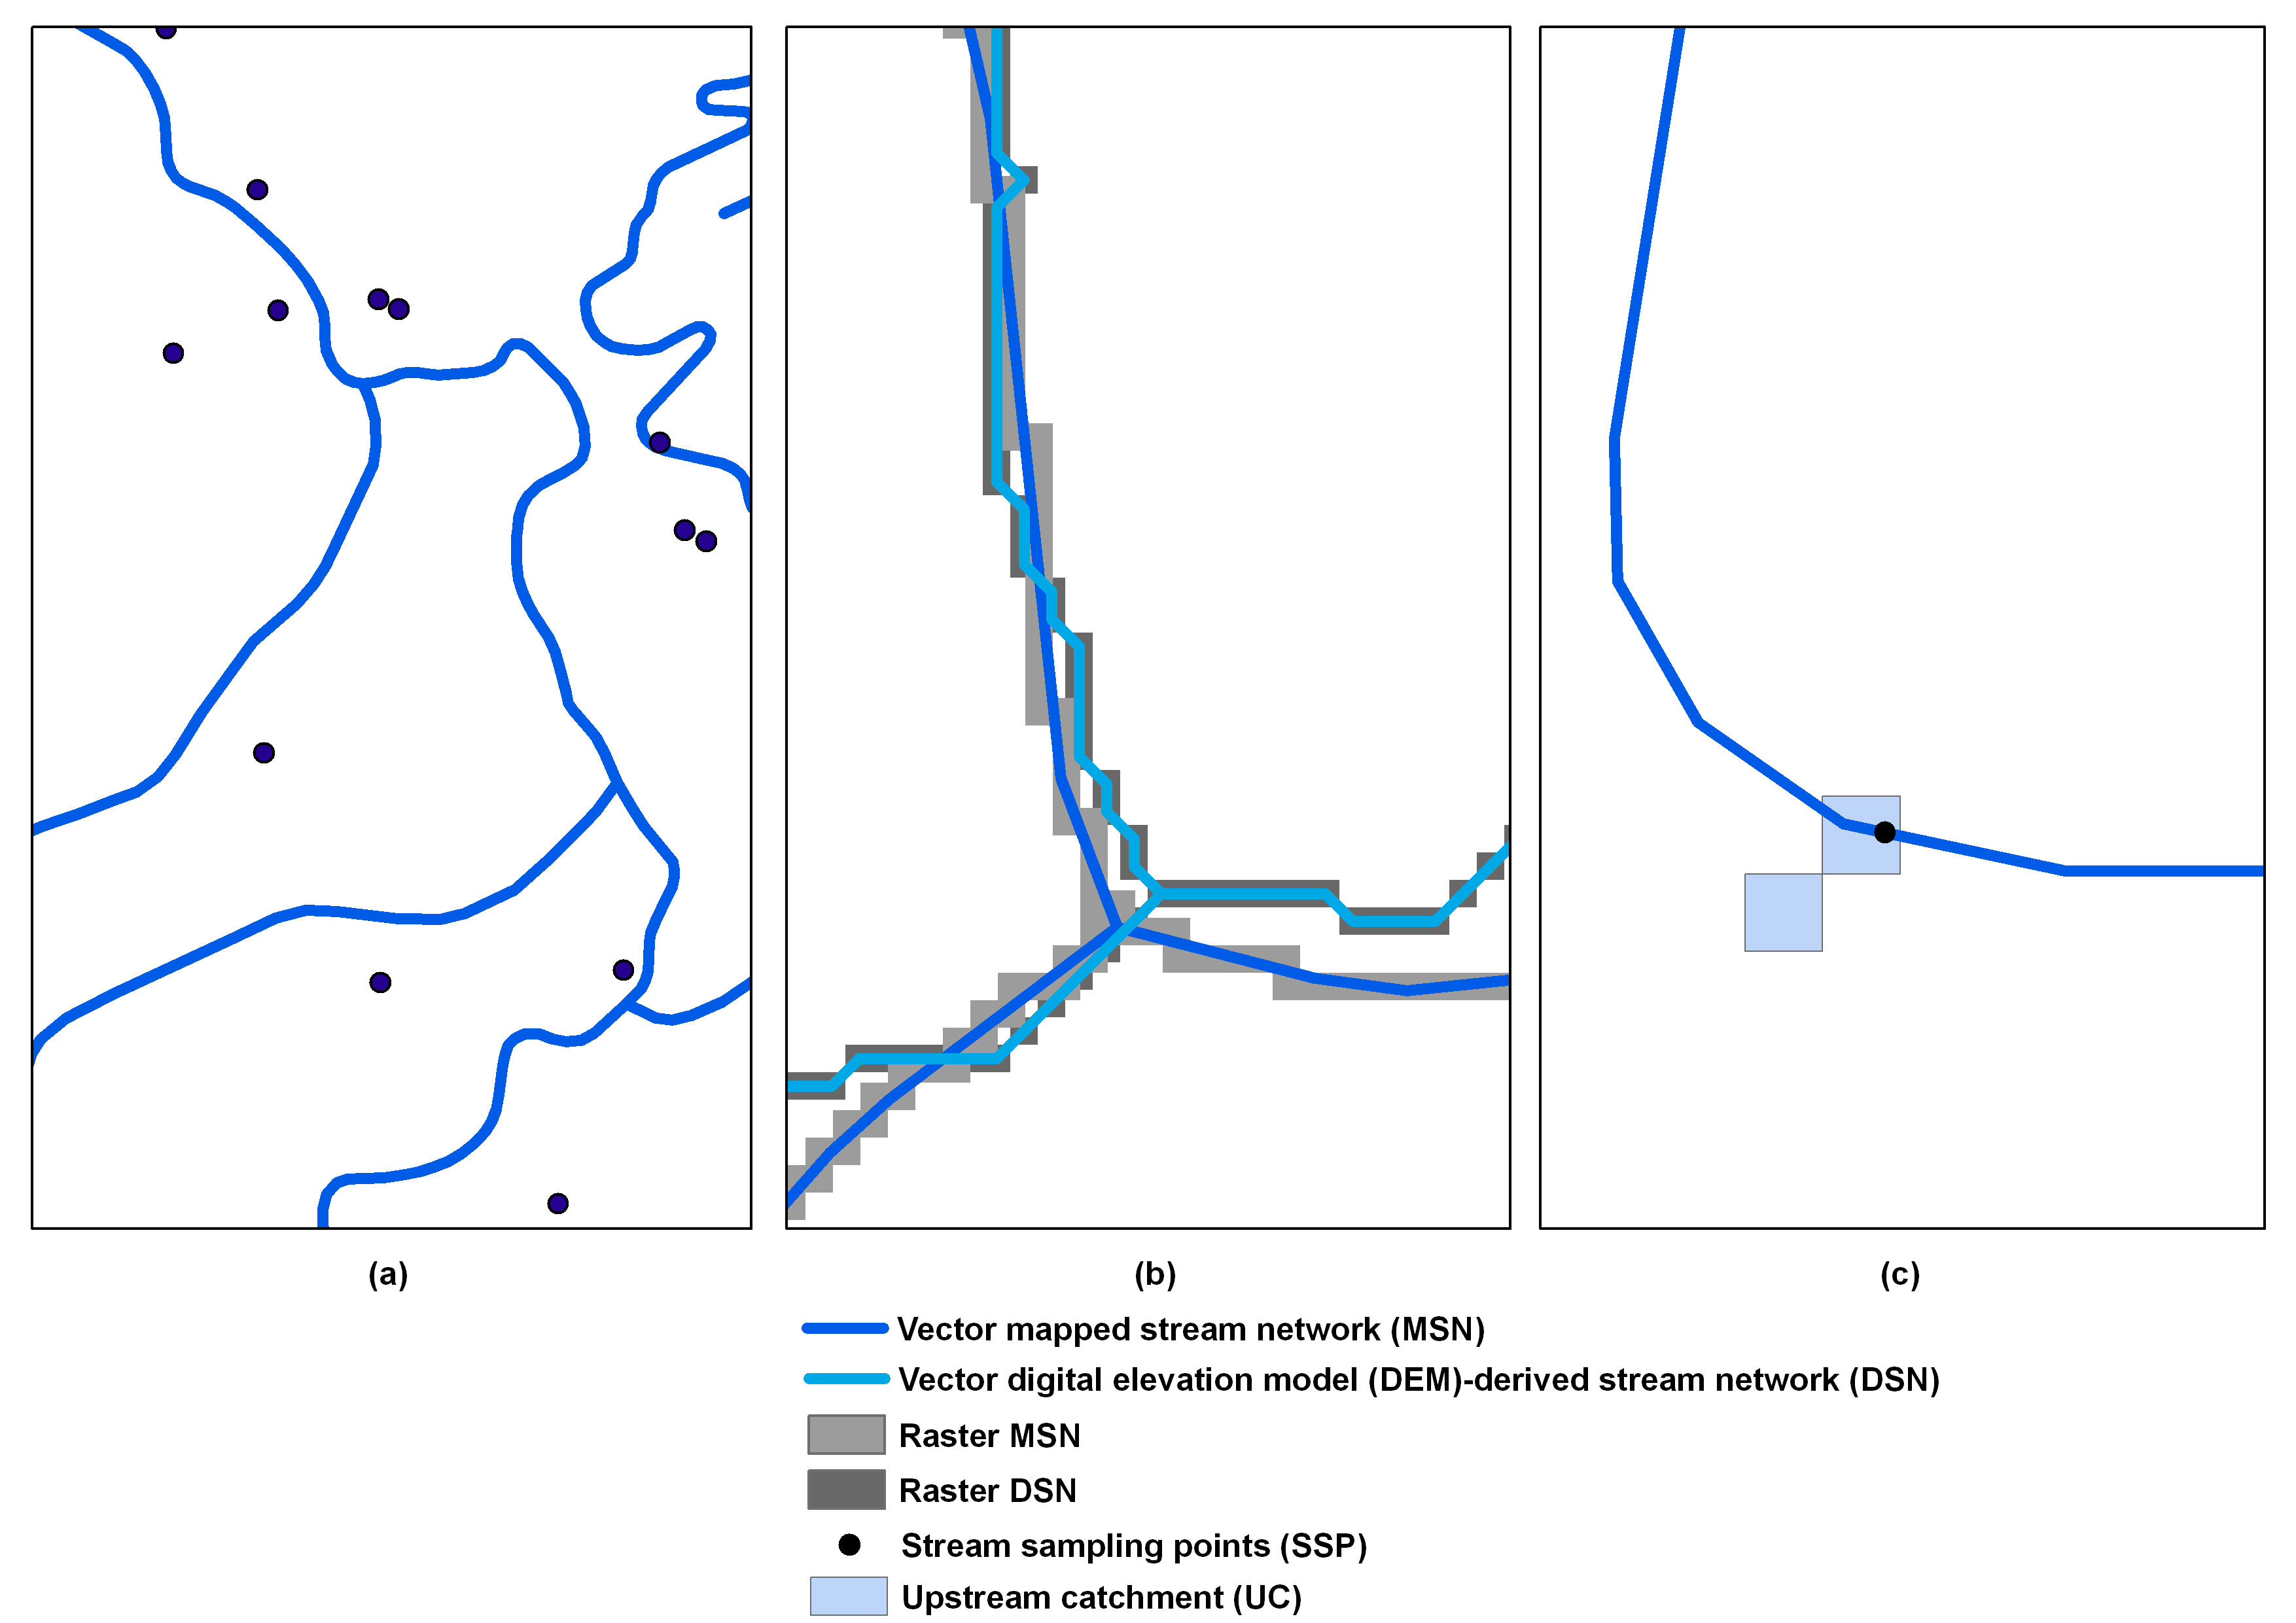
\includegraphics[width=0.9\linewidth]{Figures/Fig_S1_3.png}
  \caption{Lateral displacements observed (a) between given stream sampling points (SSP) and mapped stream network (MSN), (b) between digital elevation model (DEM)-derived  stream network (DSN) and MSN, and (c) delineated scattered and irrelevant upstream catchment for SSP after snapping to MSN.}
  \label{Fig_A_3}
\end{figure}

\end{landscape}